\cotefile{10}
\scanpage{123}

$\handwritten{\unsure{\pi|\tau}}_i^{\handwritten{2}}=\handwritten{\pi}_i,\handwritten{\pi}_i\handwritten{\pi}_j=0$ pour $i\handwritten{\ne}j$, $\handwritten{\sum_i\pi}_i=1$. La donnée d'une $\otimes$-structure sur $C$ \deleted{c}impliquant les données a)b),et celles-ci compatibles avec le foncteur $C\handwritten{\to}D$ (pour $c=\mathrm{id}$),équivaut alors à une structure d'algèbre associative unitaire sur $A$, \deleted{p}compatible avec la structure de coalgèbre, et pour laquelle $A\handwritten{\to}k\handwritten{[}T,T^{-1}\handwritten{]}$ est un homomorphisme d'\deleted{\unsure{d|i}}algèbres. Comment s'exprime le fait que \deleted{$C\unsure{\to}D$ est} sur $C$ il y a une structure de symmétrie \deleted{telle} respectée par le foncteur $C\handwritten{\to}D$ (et $c$ choisi plus haut) ? On peut d'abord exprimer la structure\inserted{\handwritten{$\otimes$}\handwritten{\begin{tikzpicture}[x=.4cm,y=.4cm,baseline=-.2ex]\draw (0,-.35) .. controls (.10,-.05) and (.20,.20) .. (.38,.42);\end{tikzpicture}}} précédente par une application diagonale de $U$ satisfaisant $\handwritten{\Delta}(\handwritten{\pi}_i)=\handwritten{\sum}_{j+k=i}\handwritten{\pi}_j\otimes\handwritten{\pi}_k$. \deleted{C}La condition cherchée \deleted{revient à dire que si $M$ est un $U$-module de degré $i$, \unsure{\deleted{N}i|\deleted{I}N|N}.e. tel que ${}_iM=M$, et $N$ de degré $j$ i.e. ${}_jN=N$, alors l\deleted{a}'isomorphisme $x\otimes y\quad(-1)^{ij}y\otimes x$ de $M\otimes_kN$ sur $N\otimes_kM$ est compatible avec les opérations de $U$} est celle-ci: si nous graduons $U$ par ``degré des opérateurs dans des gradués'' i.e. \deleted{$U^i\unsure{=\sum_j|=\pi_j|=U_j}$} ces quotients $U_{\handwritten{\alpha}}$ par $U_{\handwritten{\alpha}}^i=\handwritten{\widehat{\sum}\pi}_{i+j}U_{\handwritten{\alpha}}\handwritten{\pi}_i$, alors l'application diagonale devient \uline{anti}commutative i.e. la \unsure{mu\deleted{t}l\deleted{l}tiplication|mu\deleted{l}t\deleted{t}liplication} de $A$ \deleted{respecte} est \uline{anticommutative}. (Il y aurait lieu de prouver que la graduation de $A$\inserted{i.e. de $U$\handwritten{\begin{tikzpicture}[x=.45cm,y=.45cm,baseline=-.2ex]\draw (0,-.35) .. controls (-.06,.05) and (.18,.13) .. (.40,.15)--(2.0,.15) .. controls (2.22,.16) and (2.40,.20) .. (2.41,.42);\end{tikzpicture}}} permet de récupérer l\deleted{e}a \deleted{foncteur \unsure{ou|au|du}} \deleted{f}graduation sur le foncteur oubli,\margin{à \deleted{r}vérifier, \handwritten{(\unsure{groupe|gr. $-\nu-$} \unsure{de|des|les} classes quelc. \unsure{pour|par} \unsure{gr.duation|graduation} ?)}} i.e. les $\handwritten{\pi}_i\handwritten{\in}U$ i.e. $A\handwritten{\to}k\handwritten{[}T,T^{-1}\handwritten{]}$, et que la graduation de $A$ \deleted{n'est} peut être choisie arbit\unsure{\deleted{r}a|\deleted{a}r}i\unsure{\deleted{e}r|\deleted{r}e}ement, avec la seule condition, de toutes façons nécessaire\deleted{s}, que $A$ soit anticommutative et l'homomorphisme diagonal \deleted{es}\handwritten{soi}t compatible aux graduations).

\handwritten{9\unsure{/|)}} Quelles que soient les structures a)\deleted{b)}c) en jeu\inserted{(b) -l'unité - étant \deleted{fix}\handwritten{\unsure{fix|fixe|fixée}}\handwritten{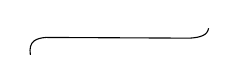
\begin{tikzpicture}[x=.45cm,y=.45cm,baseline=-.2ex]\draw (0,-.35) .. controls (-.06,.04) and (.17,.12) .. (.44,.14)--(4.5,.12) .. controls (4.8,.14) and (5.0,.20) .. (5.03,.40);\end{tikzpicture}}}, le groupe des $\otimes$-automorphismes du foncteur \deleted{fibre} ``oubli'' en est indépendant, c'est le groupe des $g\handwritten{\in}U$ tels que $\handwritten{\Delta}(g)=g\otimes g$ et d'augmentation 1,\inserted{\handwritten{(i.e. les hom unitaires $\unsure{g|q}:A\to k$)}\handwritten{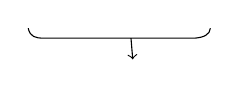
\begin{tikzpicture}[x=.45cm,y=.45cm,baseline=-.2ex]\draw (0,.28) .. controls (.05,.04) and (.20,.0) .. (.44,.0)--(4.7,.0) .. controls (4.95,.02) and (5.13,.10) .. (5.14,.28);\draw[->] (2.9,0)--(2.95,-.60);\end{tikzpicture}}}\unsure{(}NB cette dernière condition exprime la condition b) de 3º). Remplaçant $k$ par un e algèbre quelconque, on trouve encore un \deleted{foncte} schéma en monoïdes affine sur $k$, mais qui en général ne permettra pas de réconstitu\deleted{t}er la situation entièrement. \deleted{(donner exemple} Il faut analyser de plus près
